\lstset{basicstyle=\ttfamily,
	showstringspaces=false,
	commentstyle=\color{red},
	keywordstyle=\color{blue},
	frame=single
}
\lstdefinelanguage{JavaScript}{
	keywords={typeof, new, true, false, catch, function, return, null, catch, switch, var, if, in, while, do, else, case, break},
	keywordstyle=\color{blue}\bfseries,
	ndkeywords={class, export, boolean, throw, implements, import, this},
	ndkeywordstyle=\color{darkgray}\bfseries,
	identifierstyle=\color{black},
	sensitive=false,
	comment=[l]{//},
	morecomment=[s]{/*}{*/},
	commentstyle=\color{purple}\ttfamily,
	stringstyle=\color{red}\ttfamily,
	morestring=[b]',
	morestring=[b]"
}

\lstset{
	language=JavaScript,
	backgroundcolor=\color{lightgray},
	extendedchars=true,
	basicstyle=\footnotesize\ttfamily,
	showstringspaces=false,
	showspaces=false,
	tabsize=2,
	breaklines=true,
	showtabs=false,
	captionpos=b
}

\apendice{Documentación técnica de programación}

\section{Introducción}
En este apéndice se va a definir todo aquello que es necesario conocer para que se pueda continuar con el desarrollo del proyecto, desde su estructura hasta una breve descripción de como instalar la aplicación y configurar nuestro entorno de trabajo para llevar a cabo el desarrollo.

\section{Estructura de directorios}\label{cap:Estructura}
En este proyecto, aunque al principio se siguieron distintos tutoriales sobre cómo crear la estructura de directorios y ficheros, al final se optó por la opción que propone Azure. De este modo, a la hora de realizar el despliegue no tendríamos ningún tipo de problema, ya que esta plataforma requiere determinados ficheros de configuración que se explicarán a continuación.
La estructura del proyecto se divide en:


FIXME: va el dictree de abajo, pero al ponerlo dentro de un begin{figure} para que salga en una pag entera, lo mueve abajo.
\begin{figure}

\dirtree{%
	.1 / Directorio raíz.
	.2 Documentación/ - Documentación del proyecto.
	.3 img/ - Imágenes de la documentación.
	.3 tex/ - Secciones de la documentación.
	.3 anexos.pdf - Anexos del proyecto.
	.3 memoria.pdf - Memoria del proyecto.
	.2 HolaMundo/ - App web básica.
	.2 Metrominuto/ - Directorio del proyecto web.
	.3 metrominuto\_app/ - Aplicación web.
	.4 main/ - Directorio que inicializa el blueprint de la aplicación.
	.5 init.py - Inicialización.
	.5 forms.py - Contiene los formularios de la aplicación.
	.5 routes.py - Contiene las rutas de la aplicación.
	.4 static/ - Ficheros JavaScript.
	.5 css/ - Estilos.
	.5 img/ - Imágenes.
	.4 templates/ - Ficheros HTML.
	.5 ayuda - Template para la página de ayuda.
	.4 utils/ - Decoradores de la aplicación.
	.4 init.py - Inicializa la aplicación.
	.4 models.py - Clases definidas en la aplicación.
	.4 calculateRoute.py - Operaciones con el API de Google.
	.4 globals.py - Variables globales del proyecto.
	.4 graphs.py - Operaciones con grafos.
	.4 svgfunctions.py - Operaciones para dibujar.
	.4 webapp.py - Punto de entrada para la aplicación en Azure.
	.3 config.py - Fichero de configuración.
	.3 metrominuto.py - Punto de entrada para iniciar la aplicación.
	.3 metrominuto.txt - Fichero necesario para desplegar en Azure.
	.3 requirements.txt - Dependencias necesarias para ejecutar el proyecto.
}
\end{figure}
\section{Manual del programador}
En este apartado se explican los puntos a tener en cuenta por futuros desarrolladores que tengan la intención de mantener o mejorar el proyecto.
\subsection{Dibujado de grafos}
El principal objetivo de este proyecto se basa en obtener un grafo final de manera que éste sea fácilmente entendible por todos. Es por ello que a la hora de dibujar dicho grafo se plantean cuestiones y problemas como dónde colocar los textos, a que distancias, cómo orientar esos textos...

Estos problemas han resultado de gran complejidad en el desarrollo final del proyecto, ya que como mencionaba antes, es el resultado final de todo el proyecto. Para solucionar el problema de que los textos no se superpongan, tanto en las líneas o \textit{caminos}, como en los puntos o \textit{paradas}, he tenido en cuenta dos opciones:
\begin{itemize}
	\item \textbf{Discretización de las líneas:} primeramente, calculamos el cuadrado o rectángulo que contiene al texto. Una vez lo hemos calculado, el método consiste en dividir los arcos del grafo en varios puntos separados una distancia $\delta$, y comprobar si alguno de esos puntos está en el interior del rectángulo que hemos calculado previamente. Ese $\delta$ se calcula proyectando sobre cada recta una distancia en el eje x mínimamente inferior a la altura del texto, y para lo cuál nos hace falta calcular el ángulo entre dicha recta y la horizontal. Para cada texto comprendido en el punto medio de cada arco, se evalúan 8 distintas posiciones a cada lado del arco\footnote{\url{https://github.com/gpm0009/TFG_MetrominutoWeb/issues/91}}. Para el texto relativo a la información de cada nodo se evalúan estas posiciones para la posición inferior, superior, izquierda y derecha del nodo, y si no se encontrase ninguna se pasaría a evaluar las esquinas del cuadrado que contiene al círculo. En la figura \ref{fig:discretizacion} vemos un ejemplo de las 8 anclas en el rectángulo A. 
	\imagen{discretizacion}{Discretización.}
	Se observa cómo hay 3 puntos de la línea L2 que se solapan con el rectángulo que contiene la etiqueta A
	
	\item \textbf{Superposición de cuadrados:} al igual que en el método anterior, calculamos el cuadrado que contiene el texto. Una vez que sabemos esto, podemos construir varios rectángulos en torno al punto donde queremos colocar el texto, tanto a un lado de la línea como al otro. Posteriormente, dividiremos la línea que une los dos puntos para los que queremos colocar el texto en cuatro cuadrados partiendo del punto medio. De este modo, en dos de ellos la diagonal sería parte de la línea que une los puntos, mientras que en los otros dos no habría nada. De este modo, y conociendo la dirección de la línea podemos calcular si, sobre los rectángulos que forman parte de la línea, existe una superposición con alguno de los posibles rectángulos del texto. En el caso del texto que referencia el punto, el rectángulo, o en este caso cuadrado, que se construye sería el que contiene al círculo y se evaluaría el rectángulo correspondiente del que la línea forma parte. En la figura \ref{fig:rectangulos-metodo} vemos un ejemplo: los rectángulos que contienen a la línea serían B, D, H y F, mientras que los rectángulos A, C, E y G no. Por ello, siempre que el rectángulo se encuentre dentro del segundo grupo no tendremos problemas de superposición con las líneas.
	\imagen{rectangulos-metodo}{Superposición de rectángulos.}
\end{itemize}
Finalmente, se optó por la primera opción, ya que después de comprobar que los textos no se superponían con las líneas, había que tener en cuenta que no se superpusiesen entre ellos. Para ello, sobre la lista de puntos discretizados, se añaden las 4 esquinas de los rectángulos que contienen al texto. Con esta operación lo que hacemos es que si, al colocar el siguiente texto en una de las posiciones establecidas, nos encontramos con que uno de estos puntos está en el interior de este último rectángulo, significará que ya hay un texto en esa posición y debemos probar con la siguiente.

Un aspecto clave, y a tener muy en cuenta en la evaluación de todo lo comentado anteriormente, es que en todo momento estos cálculos se hacen para dibujar en SVG, por lo que el punto mas pequeño de la <<coordenada $x$>> y de la <<coordenada $y$>> se encuentra en la esquina superior izquierda. Esto nos lleva a que cada posible ancla (punto inferior izquierdo) del rectángulo del texto debemos restarle la altura de dicho texto para que la evaluación de los puntos coincida, ya que al dibujarlo en SVG el texto siempre se dibuja hacia arriba desde el punto que indicamos. Para entender mejor esto, los puntos \textit{A} y \textit{C} de la imagen~\ref{fig:rectangulos} corresponderían con el punto inferior izquierdo del rectángulo que queremos evaluar, mientras que los puntos \textit{B} y \textit{D} serían los puntos que debemos indicar al dibujar el SVG.
\imagen{rectangulos}{Puntos del rectángulo.}


\section{Aplicaciones utilizadas}
Para el desarrollo de este proyecto se han usado diferentes herramientas para incluir distintas funcionalidades, las cuales se explican brevemente a continuación:

\begin{itemize}
	\item \textbf{Visual Studio Code}: se ha utilizado para el despliegue de la aplicación en Azure, ya que desde el editor es más cómodo.
	\item \textbf{PyCharm}: se ha utilizado para el desarrollo de la aplicación. Acceso a licencia profesional con el correo de la Universidad.
	\item \textbf{GitHub}: como sistema de gestión y control de versiones del proyecto.
	\item \textbf{GitCraken}: al principio del proyecto se utilizó para realizar las subidas de los cambios en el proyecto al repositorio de GitHub, pero al final se usó la integración con GitHub de PyCharm.
	\item \textbf{Lucidchart}\footnote{\url{https://app.lucidchart.com}}: se ha utilizado para realización de los diagramas de casos de uso, secuencia...
	\item \textbf{Adobe illustrator}: se utilizó la versión de prueba para la realización del logo de la aplicación.
	\item \textbf{TeXstudio}: herramienta utilizada a lo largo del proyecto para realizar la documentación.
	\item \textbf{Google console}: herramienta utilizada para la administración y gestión de los servicios de la API.
	\item \textbf{Firebase console}: herramienta utilizada para la administración y gestión de la autenticación en la aplicación.
\end{itemize}
Después de analizar y configurar ambos editores de texto, se llegó a la conclusión de que era mucho mas cómodo y útil utilizar PyCharm, ya que ofrece una configuración mas sencilla, además de permitir importar diversas librerías de una manera mas amigable. También ofrece la posibilidad de seguir los estándares de programación \textit{PEP8} y \textit{ECMAScript}.
Para el control de versiones se ha utilizado GitCraken al comienzo del proyecto. Después, se utilizó la funcionalidad integrada en el propio IDE de desarrollo.


\section{Instalación y configuración}
Para la instalación del proyecto se explicarán los pasos a seguir en un sistema operativo de Linux, que en este caso se trata de la versión Linux Mint 18.3 Sylvia.
Tras varias pruebas, la instalación y ejecución del proyecto es idéntica salvo la propia instalación de Pycharm y Python.

\subsection{Python}

Este proyecto está desarrollado con la versión 3.6.3. Python se puede descargar desde el siguiente enlace: 
\url{https://www.python.org/downloads/}

\subsection{Instalación y configuración de PyCharm}
Este \textit{IDE} tiene distribución para Linux, además de permitir a estudiantes usar la versión profesional. Para su instalación podemos usar la \textit{snap store} de Linux, que en caso de no tenerla instalada tenemos que ejecutar el siguiente comando:

\renewcommand{\lstlistingname}{Instalar PyCharm}% Listing -> Algorithm
\renewcommand{\lstlistlistingname}{List of \lstlistingname s}
\begin{lstlisting}[language=bash,caption={Instalar snapd}]
$ sudo apt update
$ sudo apt install snapd
\end{lstlisting}

Después de tener instalado esto, ejecutaríamos:
\begin{lstlisting}[language=bash,caption={Instalar PyCharm}]
$ sudo snap install 
	pycharm-community|professional --classic
\end{lstlisting}

Una vez instalado \textit{PyCharm}, la forma más cómoda de obtener el código del proyecto es mediante \textit{git}, usando para ello el comando:

\renewcommand{\lstlistingname}{Configurar PyCharm}% Listing -> Algorithm
\renewcommand{\lstlistlistingname}{List of \lstlistingname s}
\begin{lstlisting}[language=bash,caption={Descargar el repositorio}]
$ git clone <url_del_repositorio>
\end{lstlisting}
Siendo \url{https://github.com/gpm0009/TFG_MetrominutoWeb.git} la URL del repositorio.

Para instalar las dependencias ejecutar el comando:
\begin{lstlisting}[language=bash,caption={Instalar requirements.txt}]
$ pip install -r requirements.txt
\end{lstlisting}

\subsection{Claves de Google}\label{cap:google}
Para la obtención de una \textit{Google API KEY} es necesario obtener los credenciales en  \url{https://console.developers.google.com/apis/credentials}.\\
Una vez registrados en Google, en el caso de que no lo estuviésemos ya, debemos acceder a la \textit{consola}\footnote{\url{https://console.cloud.google.com}} y desplegar el panel de la parte izquierda.
\imagen{panelGoogle}{Panel Google Console}

Hacemos click sobre <<APIs y servicios>> - <<Credenciales>> y después sobre la clave que se nos ha generado anteriormente. Desde el apartado <<Restricciones de API>> podremos seleccionar que servicios queremos que proporcione nuestra clave y restringir desde dónde se va a usar. En concreto, para este proyecto debemos tener activados:
\begin{itemize}
	\item Directions.
	\item Distance Matrix.
	\item Geocoding.
	\item Maps JavaScript.
	\item Places.
\end{itemize}


Una vez que la tenemos, debemos incluirla en el proyecto. Para ello:
\renewcommand{\lstlistingname}{Google Key}% Listing -> Algorithm
\renewcommand{\lstlistlistingname}{List of \lstlistingname s}
\begin{lstlisting}[language=python,caption={Añadir \texttt{API\_KEY}}]
google_maps=googlemaps.Client(key='GOOGLE_API_KEY')
\end{lstlisting}

Además, no hay que olvidar incluirla en los templates:
\begin{lstlisting}[language=html,caption={Añadir \texttt{API\_KEY} a los templates}]
<script
 src="https://maps.googleapis.com/maps/api/
	 js?key=API_KEY&libraries=places" 
	 type="text/javascript"</script>
\end{lstlisting}

También podemos incluirla como variable de entorno en nuestro editor. De esta manera nos aseguramos de no compartirla al realizar los commits en el control de versiones. En este caso, en PyCharm se configura de la siguiente manera:
\begin{enumerate}
\item Abrir selector Run Configuration (arriba a la derecha)
\item Edit Configurations...
\item Environmental variables
\item Add or change variables, then click OK 
\end{enumerate}


\subsection{FirebaseUI Auth}
Para la obtención de las claves de autenticación con FirebaseUI\footnote{\url{https://github.com/firebase/firebaseui-web\#configuration}} en nuestro proyecto debemos seguir los siguientes pasos:

\begin{steps}
	\item Loguearnos en Firebase con nuestro usuario de Google, preferiblemente el mismo usuario que para la configuración del apartado~\ref{cap:google}.
	\item \textit{Agregar un proyecto}. En este paso debemos elegir el proyecto creado en el apartado~\ref{cap:google}. Nos añadirá el plan de pago por defecto, ya que el proyecto que hemos escogido tiene asociado este plan para poder usar las APIs de los mapas. Se agregará automáticamente una API\_KEY a nuestra consola de Google, a la cual, deberemos restringir su uso para \textit{Identity Toolkit API}.
	\item Se abrirá automáticamente la página de descripción general del proyecto. Hacer click sobre \textit{Agregar Firebase a tu app web}, y seleccionar \textit{web}.
		\imagen{AñadirAppFirebase}{Firebase: Añadir Aplicación.}
\end{steps}


  
\subsection{\TeX studio}
Esta herramienta para la compilación de documentación \LaTeX{} permite la instalación de diccionarios para aplicar las reglas al texto. Para ello, debemos acceder a:

\renewcommand{\lstlistingname}{Configure \TeX studio}% Listing -> Algorithm
\renewcommand{\lstlistlistingname}{List of \lstlistingname s}
\begin{lstlisting}[language=bash,caption={Añadir diccionario}]
Options -> Configure TeXstudio
Language checking
\end{lstlisting}

Una vez ahí, vemos que nos ofrece dos opciones para buscar diccionarios: \url{https://extensions.openoffice.org/de/search?f[0]=field_project_tags} o \url{https://extensions.libreoffice.org/extensions?getCategories=Dictionary&getCompatibility=any}. Elegimos cualquiera de ellas y descargamos el paquete del diccionario que queramos, y después lo importamos.


\section{Bibliotecas y Frameworks}

\subsection{NetworkX}\label{networkx}
Como ya he mencionado, esta biblioteca nos permite trabajar de una forma muy amplia y completa con grafos~\cite{doc:networkx}. A lo largo del proyecto se han usado:
\begin{itemize}
	\item \texttt{graph()}: para crear un grafo no dirigido al que se añadirán nodos y arcos.
	\item \texttt{add\_node()}: Diferentes nodos junto con atributos como la posición obtenida del API de Google y el nombre.
	\item \texttt{add\_edge()}: Arco que conecta dos nodos. Además, los arcos contienen atributos como la distancia real que hay de nodo a nodo o el número de votos que tendrá.
	\item \texttt{get\_edge\_attributes()}: para obtener los valores de un atributo perteneciente a los arcos. Devuelve una lista que contiene el nodo de origen, el nodo destino y el atributo deseado.
	\item \texttt{edges(data=True)}: devuelve los arcos junto con los atributos.
	\item \texttt{nodes(data=True)}: devuelve los nodos junto con los atributos.
	\item \texttt{minimum\_spanning\_edges()}: devuelve un iterador con los arcos que forman el grafo de tal manera que la suma de distancias es la mínima.
	\item \texttt{draw\_networkx()}: para dibujar el grafo.
	\item \texttt{drawconnected\_components()}: devuelve un set con los distintos subgrafos o partes conexas dentro del grafo.
\end{itemize}

Para su uso, es necesario instalar el requirement correspondiente e importarla en el proyecto. Para ello:
\renewcommand{\lstlistingname}{NetworkX}
\renewcommand{\lstlistlistingname}{List of \lstlistingname s}
\begin{lstlisting}[language=python,caption={Instalación mediante pip.}]
pip install networkx
\end{lstlisting}
\begin{lstlisting}[language=python,caption={Importación.}]
import networkx
\end{lstlisting}

\subsection{SVGWRITE}\label{svgwrite}
\textit{Svgwrite} permite crear en el servidor nuevos archivos SVG~\cite{doc:svgwritedocs}. Permite crear, dentro del dibujo SVG distintos elementos, siendo en el caso de este proyecto círculos, rectángulos, líneas y textos. 

Para su uso, debemos instalar el \textit{requirement} e importarla al proyecto:
\renewcommand{\lstlistingname}{SVGWRITE}
\renewcommand{\lstlistlistingname}{List of \lstlistingname s}
\begin{lstlisting}[language=python,caption={Instalación mediante pip.}]
pip install svgwrite
\end{lstlisting}
\begin{lstlisting}[language=python,caption={Importación.}]
import svgwrite
\end{lstlisting}

Para el dibujado hacemos uso del método \texttt{Drawing()}, del cual dependerán todos los elementos que queramos añadir. Un ejemplo de uso sería:
\begin{lstlisting}[language=python,caption={Ejemplo de uso.}]
dwg = svgwrite.Drawing(file_name, size=('100%', '100%'), viewBox='0 0.2 1 1.5', profile='full')
line = dwg.line(id=id_edge,
	start=(start[0], start[1]),
	end=(end[0], end[1]),
	stroke='black', fill='red', stroke_width=1, class_='static')
dwg.add(line)	
dwg.save(pretty=True)
\end{lstlisting}



\subsection{SNAP.SVG}\label{snapsvg}
\textit{Snap.svg} es otra librería para crear gráficos vectoriales pero esta vez en la parte del cliente gracias a que es una biblioteca JavaScript~\cite{doc:snapsvg}. Esto la hace perfecta para manipular los elementos del SVG a nuestro antojo sin tener que hacer nuevas llamas al servidor.

Para su uso debemos incluirla en el proyecto siguiendo una de las opciones propuestas en su documentación\footnote{\url{https://github.com/adobe-webplatform/Snap.svg}} de GitHub. En este proyecto, se ha optado por descargar el directorio \texttt{\textbackslash{dist}} e incluir los ficheros JavaScript en el proyecto.

Una de las razones principales por las que he usado esta biblioteca es porque permite asociar las líneas o <<path>> que unen dos puntos con dichos puntos, y, por lo tanto, si definimos una función para mover los puntos la posición de las líneas se actualiza sin necesidad de realizar cálculos adicionales.
\renewcommand{\lstlistingname}{Snap.svg}
\renewcommand{\lstlistlistingname}{List of \lstlistingname s}
\begin{lstlisting}[language=javascript,caption={Ejemplo}]
var s = Snap("#svg");
// Crear un circulo.
var bigCircle = s.circle(150, 150, 100);
// Cambiar el color.
bigCircle.attr({
fill: "#bada55",
stroke: "#000",
strokeWidth: 5
});
\end{lstlisting}


\subsection{Jquery}\label{cap:jquery}
\textit{Jquery~\footnote{\url{https://jquery.com/}}} es una biblioteca JavaScript que permite la manipulación de documentos HTML, así como sus eventos. Para importarla a nuestro tenemos dos opciones, descargar el código e importarlo en el documento HTML desde nuestro directorio \verb|/static/js|, o incluir el \textit{CDN} al principio del documento.
\renewcommand{\lstlistingname}{Jquery}
\renewcommand{\lstlistlistingname}{List of \lstlistingname s}
\begin{lstlisting}[language=javascript,caption={Jquery cdn.}]
<script src="https://code.jquery.com/jquery-3.4.1.slim.min.js"
	integrity="sha384-J6qa4849blE2+poT4WnyKhv5vZF5SrPo0iEjwBvKU7imGFAV0wwj1yYfoRSJoZ+n"
	crossorigin="anonymous">
</script>
\end{lstlisting}

\subsection{Vue.js}\label{cap:Vue}
\textit{Vue}~\cite{doc:vue} es un framework de JavaScript diseñado para la elaboración de interfaces de usuario. Para trabajar con este framework en el proyecto es necesario añadir en el template su cdn~\footnote{\url{https://es.vuejs.org/v2/guide/installation.html}}, o como alternativa descargar el código e importarlo desde nuestro directorio \verb|/static/js|.
\renewcommand{\lstlistingname}{Vue.js}
\renewcommand{\lstlistlistingname}{List of \lstlistingname s}
\begin{figure}
\begin{lstlisting}[language=javascript,caption={Vue cdn.}]
<!-- version de desarrollo, incluye advertencias de ayuda en la consola -->
<script src="https://cdn.jsdelivr.net/npm/vue/dist/vue.js"></script>
<!-- version de produccion, optimizada -->
<script src="https://cdn.jsdelivr.net/npm/vue"></script>
\end{lstlisting}
\end{figure}

Además debemos crear un componente\footnote{\url{https://vuejs.org/v2/guide/components.html}}, al que le añadiremos una variable, que hará referencia al \verb|<div>| donde queremos incluirlo. Esto se debe a que realmente la estructura y el nombre de los elementos de Vue es algo diferente a los que ya conocemos de \textit{HTML5}. También es importante tener en cuenta que Vue utiliza los mismos delimitadores que \textit{Flask}: \verb|{{variable}}|. Es por esto por lo que a nuestro componente o variable debemos añadir la línea \verb|delimiters:['[[',']]']| para cambiarlos.

También es recomendable instalar las extensiones de desarrollo, bien sea para Chrome~\footnote{\url{https://chrome.google.com/webstore/detail/vuejs-devtools/nhdogjmejiglipccpnnnanhbledajbpd}} o para Firefox~\footnote{\url{https://addons.mozilla.org/en-US/firefox/addon/vue-js-devtools/}}, ya que a la hora de desarrollar el proyecto permiten inspeccionar los elementos desde la consola del navegador.

\subsection{FirebaseUI}\label{firebase}
Para incluir la configuración de Firebase en el proyecto, seguir estos pasos:
\begin{enumerate}
	\item Acceder a la configuración general del proyecto e ir a \textit{Tus aplicaciones}.
	\item Copiar el apartado \textit{Firebase SDK snippet} y pegarlo en el fichero de configuración del proyecto \verb|/Metrominuto/metrominuto_app/static/js/firebase-config.js|.
	\item Añadir en el template \textit{widget.html} los proveedores que queramos.
\end{enumerate}

Además, cuando el acceso se realiza correctamente, Firebase permite ver la información básica del perfil. También permite una administración y control total de dichos accesos, ya que en todo momento podemos saber quién esta accediendo a la app, como vemos en la siguiente figura:
\imagen{Firebase-users}{Control de usuarios.}

\section{Compilación, instalación y ejecución del proyecto}
Para el desarrollo de este proyecto se ha usado PyCharm, por lo que esta guía esta orientada a este editor. Para Visual Studio Code puede visitarse el enlace \url{https://code.visualstudio.com/docs/python/tutorial-flask}, ya que la creación y ejecución del entorno virtual no es igual.

\subsection{Python}
Este proyecto está desarrollado con la versión 3.7.5, pero con para desarrollar la mínima es 3.6. Python se puede descargar desde el siguiente enlace: \url{https://www.python.org/downloads/}.

\subsection{Instalación}
La forma más cómoda de obtener todo el proyecto es mediante \textit{git}, usando el comando:
\renewcommand{\lstlistingname}{Instalación}% Listing -> Algorithm
\renewcommand{\lstlistlistingname}{List of \lstlistingname s}
\begin{lstlisting}[language=python,caption={Descargar el repositorio.}]
 $ git clone <url_del_repositiorio>
\end{lstlisting}
Siendo \url{https://github.com/gpm0009/TFG_MetrominutoWeb} la URL del repositorio en \textit{GitHub}. Ya con el proyecto descargado, el siguiente paso es instalar las dependencias. Aunque se pueden instalar sobre la instalación global de Python, es recomendable usar un entorno virtual. Para ello, debemos abrir el directorio del proyecto desde Pycharm, y una vez que lo tengamos ir a \textit{Files - Settings - Project Interpreter - Add}, y seleccionar la opción de \textit{Virtual Envirorment} y a continuación creamos uno nuevo.
\imagen{NewVirtualEnvirorment}{Creación del entorno virtual.}
Después, el editor detectará automáticamente el fichero \textit{requirements.txt} y nos preguntará si queremos instalar las dependencias, a lo que le diremos que sí. De no ser así, hay que abrir la terminal en la parte inferior del editor y ejecutar el comando:
\begin{lstlisting}[language=python,caption={Instalar dependencias en el entorno virtual.}]
$ pip -r install requirements.txt
\end{lstlisting}

\subsection{Variables de entorno}\label{variables_entorno}
Para que la aplicación funcione correctamente hay que definir las siguientes variables de entorno:
\begin{itemize}
	\item \textbf{\texttt{GOOGLE\_API\_KEY}:} clave obtenida anteriormente necesaria para obtener datos de Google.
	\item \textbf{\texttt{SECRET\_KEY}:} clave necesaria por Flask.
	\item \textbf{\texttt{ENVIRORMENT}:} en el que se está actualmente: development o production.
\end{itemize}
Para su configuración, acceder desde la parte superior derecha del editor a \textit{Edit Configurations$\dots$} y después seleccionar \textit{Envirorment variables} como vemos en la figura~\ref{fig:envirorment_variables}.
\imagen{envirorment_variables}{Variables de entorno.}

\subsection{Ejecución}
Para la ejecución desde el editor, es necesario que hagamos una última configuración. Debemos ir a la parte superior derecha del editor y seleccionar \textit{Edit Configurations$\dots$} como se ven en la figura \ref{fig:ejecucion}.
\imagen{ejecucion}{Ejecución del proyecto.}

En esta pantalla tenemos que elegir el punto de entrada a la aplicación, que será el fichero \textit{metrominuto.py}, escribir el entorno en el que queremos ejecutar la aplicación y marcar la opción de Debug. Una vez hecho esto, ya podemos ejecutar la aplicación desde el panel superior derecho.

\subsection{Despliegue en Azure}
Para realizar el despliegue de la aplicación en Azure es necesario que el proyecto tenga una estructura concreta, ya que serán los servicios de Azure los que instalen las dependencias necesarias y ejecuten el código. Dicha estructura es la definida anteriormente en el apartado \textit{Estructura de directorios}~\ref{cap:Estructura}. Para ello he seguido el tutorial propuesto por Microsoft~\cite{deploy-flask-azure}, junto con el ejemplo de de aplicación que propone~\footnote{\url{https://code.visualstudio.com/docs/python/python-tutorial}}.

Antes de hacer el despliegue, es importante acordarse de configurar en Azure las variables de entorno que teníamos definidas~\ref{variables_entorno}. Para ello debemos entrar, en Azure, a nuestro \textit{APP Service} y añadirlas en el apartado de \textit{Configuración} que aparece en el menú desplegable de la izquierda,  véase la figura~\ref{fig:configuracion_paso1}.

\begin{figure}[!h]
	\centering
	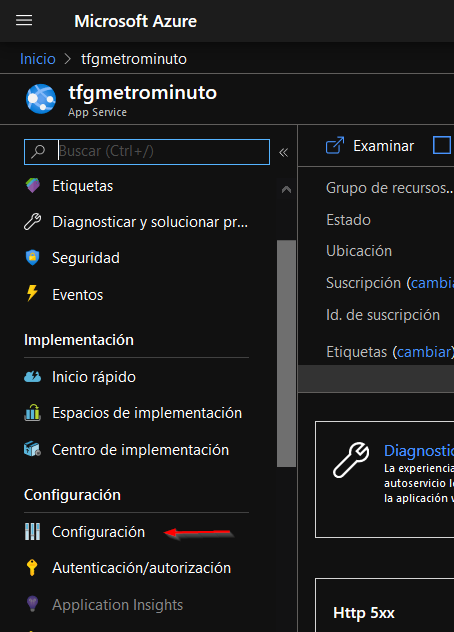
\includegraphics[width=0.7\textwidth, height=12cm]{configuracion_paso1}
	\caption{Configuración Variables de entorno en Azure, paso 1.}\label{fig:configuracion_paso1}
\end{figure}
\FloatBarrier


A continuación, seleccionar \textit{Configuración de la aplicación} y \textit{Nueva configuración de la aplicación}, como vemos en la Figura~\ref{fig:configuracion_paso2}.
\imagen{configuracion_paso2}{Configuración Variables de entorno en Azure, paso 2.}

\section{Pruebas del sistema}
Esta sección no es una parte en la que se haya hecho mucho hincapié a lo largo del desarrollo, pero se han realizado diferentes pruebas manuales y de usabilidad.
\\


A lo largo del desarrollo, con el objetivo de que Google no me cobrase por las múltiples llamadas a las APIs, guarde unos archivos \textit{JSON} con algunos ejemplos de datos que me proporcionaba Google. Se encuentran en el directorio \verb|/static|. Mediantes ejemplos (conociendo la entrada) se evaluaba cual era la salida esperada, que al principio comenzó siendo el posicionamiento correcto de los puntos sobre el SVG y, al final, acabó siendo el posicionamiento correcto de todas las líneas, puntos y textos sobre el SVG.




